\begin{frame}[standout]

    Bases de données clé-valeur

    \note{
        Cette slide annonce une famille très simple à comprendre :
        une clé permet de retrouver directement une valeur.
    }

\end{frame}

\begin{frame}{Caractéristiques des bases de données clé-valeur}

    \begin{definitionbox}
        Dans une base de données clé-valeur, les données sont stockées sous forme de \textbf{paires de clés uniques et de valeurs} correspondantes.

        La clé agit comme un \textbf{identifiant unique}, et la valeur peut être de tout type (chaîne de caractères, JSON, binaire, etc.).
    \end{definitionbox}

    \begin{noteblock}
        \begin{itemize}
            \item Très scalable avec une structure simple.
            \item Pas de schéma ou de structure rigide.
        \end{itemize}
        $\hookrightarrow$ Idéal pour stocker de grandes quantités de données avec une complexité relationnelle minimale.
        % $\Longrightarrow$ Idéal pour stocker de grandes quantités de données avec une complexité relationnelle minimale.
    \end{noteblock}

    \note{
        Une base clé-valeur, c’est comme un dictionnaire : tu cherches un mot (clé) et tu obtiens sa définition (valeur).

        La valeur peut être opaque pour la base : chaîne, nombre, document JSON
        ou données binaires. La base connaît surtout la clé et optimise son accès.
        Insister sur le compromis : simplicité et rapidité, mais peu de requêtes
        relationnelles ou de recherche dans le contenu.
    }
\end{frame}

\begin{frame}{Comment fonctionnent les bases de données clé-valeur ?}

    \begin{figure}
        \centering
        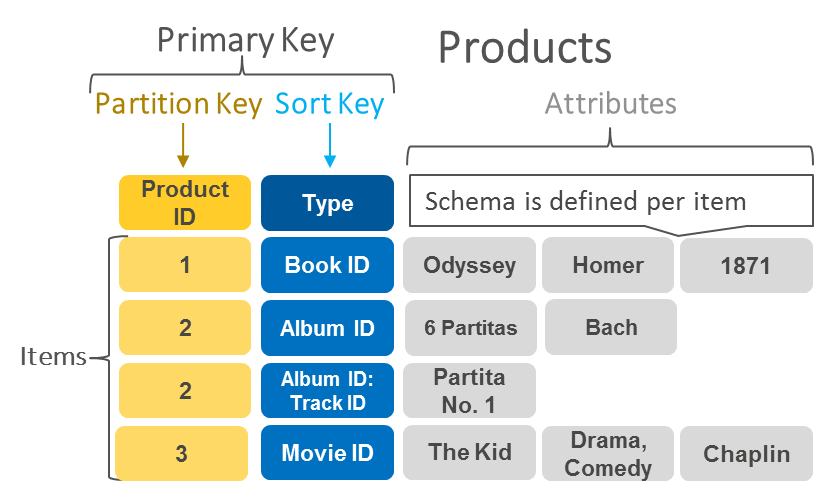
\includegraphics[width=0.8\textwidth]{img/key-value-database.png}
    \end{figure}

    \note{
        Expliquer le chemin d'accès direct : l'application fournit une clé,
        puis la base renvoie la valeur associée. Les opérations typiques sont
        GET, PUT et DELETE.
        Le modèle convient lorsque les lectures sont principalement déterminées
        par une clé connue à l'avance.
    }

\end{frame}

\begin{frame}{Bases de données clé-valeur}
    \begin{figure}[htb]
        \centering
        \begin{tikzpicture}
            \node[minimum width=3cm, minimum height=2cm] at (0, 0) {\includesvg[height=1cm]{img/db/redis.svg}};
            \node[minimum width=3cm, minimum height=2cm] at (0, -2) {\includesvg[height=1cm]{img/db/riak.svg}};
            \node[minimum width=3cm, minimum height=2cm] at (4, 0) {\includesvg[height=1cm]{img/db/memcached.svg}};
            \node[minimum width=3cm, minimum height=2cm] at (4, -2) {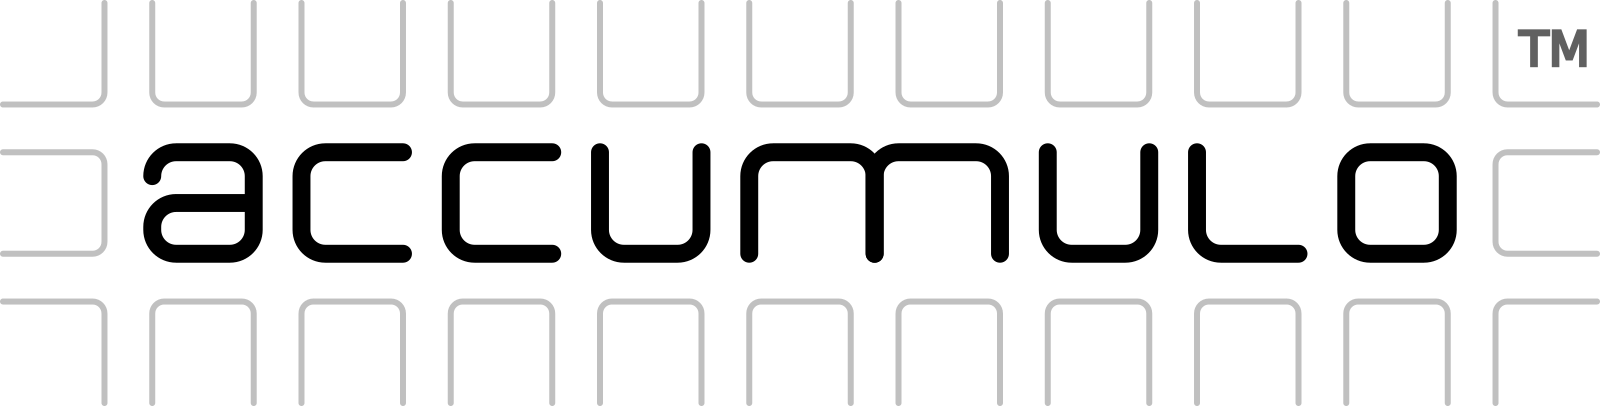
\includegraphics[height=1cm]{img/db/accumulo.png}};
            \node[minimum width=3cm, minimum height=2cm] at (0, -4) {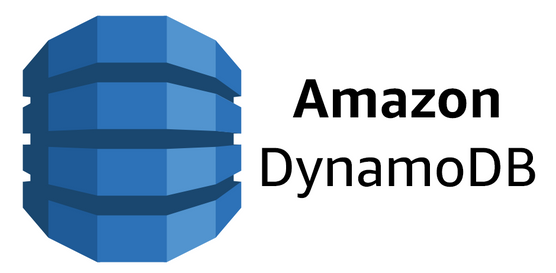
\includegraphics[height=1cm]{img/db/aws-dynamodb.png}};
            \node[minimum width=3cm, minimum height=2cm] at (4, -4) {
\includegraphics[height=1cm]{img/db/oracle-nosql.png}};
        \end{tikzpicture}
    \end{figure}

    \note{
        Ces produits partagent le modèle clé-valeur, mais leurs compromis diffèrent.
        Redis et Memcached sont souvent utilisés en mémoire et pour le cache,
        tandis que DynamoDB vise un service distribué durable.
        Il faut donc distinguer le modèle de données du produit choisi.
    }
\end{frame}


\begin{frame}{Cas d'usages des bases de données clé-valeur}
    % Gestion de session
    % Une application orientée session telle qu'une application web ouvre une session lorsqu'un utilisateur se connecte à une application,
    % puis ferme la session lorsque l'utilisateur se déconnecte ou lorsque la session expire.
    % Pendant cette période, l'application stocke tous les attributs de la session utilisateur dans la mémoire principale ou dans une base de données.
    % Les données de session peuvent inclure des informations sur le profil d'utilisateur, des messages, des données et des thèmes personnalisés,
    % des recommandations, des promotions ciblées et des remises.
    % Chaque session utilisateur possède un identifiant unique. Les données de session sont uniquement interrogées par une clé primaire.
    % Ainsi, un magasin clé-valeur rapide est idéal dans ce contexte. En général, les frais généraux par page liés aux bases de données clé-valeur
    % sont inférieurs à ceux associés aux bases de données relationnelles.

    % Panier d'achat
    % Un site Web d'e-commerce peut recevoir des milliards de commandes en quelques secondes pendant la période des achats de Noël.
    % Les bases de données clé-valeur peuvent gérer la mise à l'échelle de grandes quantités de données et de grands volumes de changements d'état
    % tout en répondant aux besoins de millions d'utilisateurs simultanés grâce à un traitement et à un stockage distribués.
    % Le stockage de données clé-valeur intègre également une capacité de redondance, ce qui lui permet de gérer la perte de nœuds de stockage.

    % Moteur de stockage des métadonnées
    % Votre stockage clé-valeur peut servir de couche de stockage sous-jacente pour des niveaux d'accès aux données plus élevés.
    % Par exemple, vous pouvez mettre à l'échelle le débit et la simultanéité pour les charges de travail multimédias et de divertissement
    % telles que le streaming vidéo en temps réel et le contenu interactif. Vous pouvez également créer votre plateforme de jeu avec les données
    % des joueurs, l'historique des sessions et les tableaux de classement pour des millions d'utilisateurs simultanés.

    % Mise en cache
    % Vous pouvez utiliser une base de données clé-valeur pour stocker temporairement des données afin de les récupérer plus rapidement.
    % Par exemple, les applications de réseaux sociaux peuvent stocker des données fréquemment consultées, telles que le contenu des fils d'actualités.
    % Les systèmes de mise en cache des données en mémoire utilisent également le stockage clé-valeur pour accélérer les réponses des applications.

    \begin{itemize}
        \item \textbf{Stockage de sessions et profils d'utilisateurs}\\
        $\hookrightarrow$ Chaque utilisateur est référencé par une clé qui permet d'accéder à ses informations.
        \vspace{0.3cm}

        \item \textbf{Paniers d'achats dans les applications de commerce électronique}\\
        $\hookrightarrow$ Gestion des commandes lors des soldes et de l'évolution de leur statut.
        \vspace{0.3cm}

        \item \textbf{Systèmes de cache (ex. : Redis, Memcached)}\\
        $\hookrightarrow$ Les applications de réseaux sociaux peuvent stocker des données fréquemment consultées, telles que le contenu des fils d'actualités.
    \end{itemize}

    \note{
        Dans une session web, l'identifiant de session est une clé naturelle.
        Pour un panier, on retrouve directement le panier d'un client et on le met
        à jour fréquemment. Le cache exploite le même principe pour éviter de recalculer
        ou de relire des données souvent demandées.
        Demander aux étudiants quel serait le choix de la clé dans chaque exemple.
    }
\end{frame}

\begin{frame}{Avantages et inconvénients des bases de données clé-valeur}
    \vfill
    \prosbox{
        \textbf{Avantages}
        \begin{itemize}
            \item Lectures et écritures extrêmement rapides grâce à l'accès direct par clé.
            \item Scalabilité horizontale facile pour de grands ensembles de données.
        \end{itemize}
    }
    \vfill
    \pause
    \consbox{
        \textbf{Inconvénients}
        \begin{itemize}
            \item Absence de requêtes complexes.
            \item Mauvaise gestion du schéma.
        \end{itemize}
    }
    \vfill

    \note{
        Résumer le choix clé-valeur ainsi : excellent quand l'application connaît
        la clé, moins adapté quand elle doit explorer ou relier les données.
        Une valeur complexe peut être stockée, mais cela ne transforme pas la base
        en moteur de requêtes document ou relationnel.
    }
\end{frame}
